\documentclass[11pt]{article}

\usepackage[T1]{fontenc}
\usepackage[utf8]{inputenc}
\usepackage{lmodern}
\usepackage[margin=1in]{geometry}
\usepackage{amsmath,amssymb,amsthm,mathtools}
\usepackage{booktabs}
\usepackage{array}
\usepackage{graphicx}
\usepackage{xcolor}
\usepackage{microtype}
\usepackage{natbib}
\usepackage{enumitem}
\usepackage{caption}
\usepackage{subcaption}
\usepackage{url}
\usepackage{xspace}
\usepackage{flafter}
\usepackage{placeins}
\usepackage[colorlinks=true,allcolors=blue!55!black]{hyperref}

\newtheorem{theorem}{Theorem}[section]
\newtheorem{proposition}[theorem]{Proposition}
\newtheorem{lemma}[theorem]{Lemma}
\newtheorem{corollary}[theorem]{Corollary}
\theoremstyle{definition}
\newtheorem{definition}[theorem]{Definition}
\newtheorem{assumption}[theorem]{Assumption}
\theoremstyle{remark}
\newtheorem{remark}[theorem]{Remark}

\newcommand{\R}{\mathbb{R}}
\newcommand{\I}{\mathcal{I}}
\newcommand{\C}{\mathcal{C}}
\newcommand{\T}{\mathcal{T}}
\newcommand{\Ph}{\mathop{\rm P}}
\newcommand{\E}{\mathop{\rm E}}
\newcommand{\ind}{\mathbf{1}}
\newcommand{\norm}[1]{\left\lVert #1\right\rVert_2}
\newcommand{\SCI}{\textnormal{\textsc{sci}}\xspace}
\newcommand{\PBP}{\textnormal{\textsc{pbp}}\xspace}

\hypersetup{
  pdftitle={Finite-Sample Confidence Sets for Nonsmooth Convex-to-Concave Transitions},
  pdfauthor={Saveliy Baturin},
  pdfsubject={Finite-sample inference for S-shaped transition locations},
  pdfkeywords={shape constraints, inflection location, finite-sample inference,
    partial identification, multiscale contrasts, S-shaped regression}
}

\title{Finite-Sample Confidence Sets for Nonsmooth\\
Convex-to-Concave Transitions}
\author{Saveliy Baturin\\Independent Researcher\\
\texttt{saveliy.xo@gmail.com}}
\date{September 2026}

\begin{document}
\maketitle

\begin{abstract}
Many scientific curves change from increasing returns to diminishing returns.
A point estimate can mark this transition, but it does not show which other
locations remain compatible with the data.  The problem is difficult when the
mean curve has a kink, a jump, or a flat transition region, because smooth
derivative and bootstrap arguments can then fail.  We introduce shape-contrast
inversion (\SCI), a finite-sample uncertainty layer for this problem.  \SCI
builds simultaneous bounds for a fixed family of local chord contrasts and
inverts only their certified signs.  The output is an outer confidence set for
all locations at which the mean curve can change from convex to concave.  In
fixed-design Gaussian regression, coverage is uniform and does not require a
derivative, continuity at the transition, or a unique transition.  We also give
finite-sample versions for unknown constant noise, bounded heteroskedasticity,
and independent replicate curves with arbitrary within-curve covariance.  In
80,000 fresh simulations, known-scale coverage ranged from 97.70\% to 98.04\%
at a 95\% nominal level across 16 published S-shaped benchmark settings.  In a
matched comparison with a generic honest confidence-region projection, \SCI
reduced median width by 19.4\%--75.7\% for cusp, onset, and jump signals.  Both
methods were wide for a weak smooth logistic signal.  Analyses of atmospheric
LIDAR and 11 replicated DNase assay runs illustrate how the answer changes with
the available noise information.  A matrix-free implementation evaluates about
six million contrasts for one million observations in less than one second on
the benchmark machine.
\end{abstract}

\noindent\textbf{Keywords:} shape constraints; inflection location;
finite-sample inference; partial identification; multiscale contrasts;
S-shaped regression.

\section{Introduction}

Researchers often need to locate a change from acceleration to saturation.
Examples include dose-response curves, biological growth, atmospheric
profiles, disease progression, and production curves.  Shape-constrained
regression can estimate such a curve without choosing a detailed parametric
model.  In particular, an S-shaped fit is convex before a transition and
concave after it \citep{feng2022sshaped}.  The fitted transition is useful, but
it does not answer a basic uncertainty question:
\begin{quote}
Which transition locations can the data rule out while remaining valid for
kinks, jumps, and flat transition regions?
\end{quote}

This is a broadly relevant data-science problem.  A reported change point is
often treated as a physical threshold or an operating decision.  If its
uncertainty method silently assumes a smooth and unique inflection, a narrow
interval can be more misleading than no interval.  The difficulty is not only
computational.  When curvature is zero over an interval, the data-generating
curve itself does not identify one preferred transition point.  A valid method
must then report a set rather than invent a unique target.

Earlier work already gives important forms of inference for qualitative
features.  \citet{davies2009nonparametric} construct finite-sample confidence
regions for a regression curve and study features including inflection points.
\citet{schmidthieber2013multiscale} use multiscale sign statements to locate
roots of operators, including curvature changes.  Shape-restricted splines and
bootstrap methods provide practical point and interval estimators under smoother
models \citep{meyer2008inference,liao2017changepoint}.  These results show that
the general topic is established and important.  Our goal is therefore not to
claim the first confidence method for an inflection point.

We address a narrower gap.  We want a direct, computable, finite-sample
confidence set for the full set of convex-to-concave transition locations.  The
validity statement should survive nonsmooth curves, nonunique transitions, and
irregular fixed designs.  The output should also be usable as an uncertainty
layer around a modern S-shaped point estimate.

Our method, shape-contrast inversion (\SCI), starts from local chord
inequalities.  A positive chord residual supports convexity on its interval; a
negative residual supports concavity.  We construct simultaneous confidence
bounds for a fixed collection of averaged residuals.  Certified positive signs
exclude transition locations to their left, while certified negative signs
exclude locations to their right.  Inverting these statements gives an outer
confidence set for every compatible transition location.

The contributions are as follows.
\begin{enumerate}[leftmargin=*,itemsep=2pt]
  \item We define the target as the full identified set of
  convex-to-concave transitions.  This makes flat transition regions explicit.
  \item We give a direct finite-sample confidence set in fixed-design Gaussian
  regression.  The theorem permits kinks, jumps, and nonunique transitions.
  \item We extend the construction to unknown constant variance, a declared
  upper bound on variance heterogeneity, and independent replicate curves with
  arbitrary within-curve covariance.
  \item We show localization under an explicit contrast-margin condition.  The
  cubic special case has the familiar $(\log n/n)^{1/7}$ order; we do not claim
  that this order is new.
  \item We give a matrix-free implementation and compare \SCI with both a
  published smooth-bootstrap method and a matched honest projection baseline.
  \item We report weak-information cases as well as successes.  A wide set is
  an intended answer when the data cannot support precise localization.
\end{enumerate}

The rest of the paper is organized as follows.  Section~\ref{sec:related}
positions the method.  Sections~\ref{sec:model}--\ref{sec:theory} define \SCI
and prove its main guarantee.  Section~\ref{sec:extensions} gives the noise
extensions.  Sections~\ref{sec:experiments} and~\ref{sec:data} report simulations
and real-data examples.  Section~\ref{sec:discussion} states the limits and the
remaining open theory.

\section{Relation to earlier work}
\label{sec:related}

\paragraph{Confidence regions and multiscale inference.}
The confidence-region approach of \citet{davies2009nonparametric} is broad: it
first constructs a set of plausible regression functions and then studies
their qualitative features.  Multiscale tests similarly turn many local
statements into global qualitative conclusions
\citep{dumbgen2001multiscale,schmidthieber2013multiscale}.  \SCI follows the
same honest-inference principle, but it targets one feature directly.  It
stores only the endpoints, scale, and sufficient sums needed for local chord
contrasts.  This direct inversion is the source of its simple proof and its
computational scale.

\paragraph{S-shaped point estimation.}
The tuning-free least-squares estimator of \citet{feng2022sshaped} estimates a
monotone S-shaped curve and its transition.  We use its implementation as the
main point estimator in our hybrid workflow.  \SCI does not replace that fit.
It supplies a confidence set around the scientific transition target.  Our
coverage theorem needs the convex-to-concave restriction but not monotonicity.

\paragraph{Spline change-point intervals.}
\citet{liao2017changepoint} estimate a change point with shape-restricted
regression splines.  Their \texttt{ShapeChange} software includes a residual
bootstrap interval.  It is a useful comparator in its smooth spline regime.
Our nonsmooth experiments deliberately include settings outside that regime,
so those comparisons measure robustness rather than a failure of the published
theory.

\paragraph{What is new here.}
The main object is a finite-sample outer confidence set for a possibly
set-valued transition under a nonsmooth shape class.  The most informative
comparison is therefore not only against a point or smooth-bootstrap method,
but also against another procedure with a matched finite-sample guarantee.
For this purpose we implement a pointwise-band projection (\PBP) baseline.  It
is related to the confidence-region strategy of
\citet{davies2009nonparametric}, but it is our deliberately simple baseline,
not their official algorithm.

\section{Model and target}
\label{sec:model}

Let
\[
  A < x_1 < \cdots < x_n < B,
  \qquad Y_i=f(x_i)+\varepsilon_i,
  \quad i=1,\ldots,n,
\]
where the design is fixed.  In the basic model,
$\varepsilon_i\stackrel{\mathrm{iid}}{\sim}N(0,\sigma^2)$ and $\sigma$ is
known.  Extensions relax the scale assumption.

\begin{definition}[Compatible transition set]
For a real-valued function $f$ on $[A,B]$, define
\[
  \I(f)=\left\{m\in[A,B]:
  f\text{ is convex on }[A,m]\text{ and concave on }[m,B]\right\}.
\]
We call every $m\in\I(f)$ a compatible convex-to-concave transition.
\end{definition}

The definition does not require a derivative.  It permits an endpoint
transition, a kink, and a one-sided jump at the transition.  It also permits a
flat-curvature interval, in which case more than one $m$ is compatible.

\begin{lemma}[Geometry of the target]
\label{lem:identified}
If $m_1<m_2$ both belong to $\I(f)$, then $f$ is affine on $[m_1,m_2]$ and
$[m_1,m_2]\subseteq\I(f)$.  Therefore, whenever $\I(f)$ is nonempty, it is an
interval, possibly a singleton.
\end{lemma}

This lemma separates statistical uncertainty from identification.  Even with
no noise, a curve that is affine over $[m_1,m_2]$ does not select one transition
inside that interval.  Our confidence statement therefore covers the whole
set $\I(f)$.

\subsection{Chord contrasts}

For design indices $L<M<R$, define the chord residual
\begin{equation}
Q_{L,M,R}(f)=
  \frac{x_R-x_M}{x_R-x_L}f(x_L)
  +\frac{x_M-x_L}{x_R-x_L}f(x_R)-f(x_M).
\label{eq:chord}
\end{equation}
Convexity makes \eqref{eq:chord} nonnegative; concavity makes it
nonpositive.  Single triples are noisy, so we average nonnegative collections
of chord residuals.  Let $\T$ be a fixed finite family.  Each
$T\in\T$ defines a row vector $w_T\in\R^n$, a support interval
$[a_T,b_T]$, and a contrast mean
\[
  Z_T=w_T^\top Y,
  \qquad \mu_T=w_T^\top f(x_{1:n}).
\]
The weights are chosen so that $\mu_T\geq0$ when $f$ is convex on the support,
and $\mu_T\leq0$ when $f$ is concave there.  The family is fixed before seeing
$Y$.  Appendix~\ref{app:contrasts} gives the construction used in the
experiments.

\section{Shape-contrast inversion}
\label{sec:method}

Let $M=|\T|$ and let $\Phi$ be the standard normal distribution function.  For
a desired error probability $\alpha$, set
\begin{equation}
  c_{\alpha,M}=\Phi^{-1}\!\left(1-\frac{\alpha}{2M}\right).
\label{eq:critical}
\end{equation}
For every contrast, form the simultaneous interval
\begin{equation}
  [\ell_T,u_T]=
  \left[Z_T-c_{\alpha,M}\sigma\norm{w_T},
        Z_T+c_{\alpha,M}\sigma\norm{w_T}\right].
\label{eq:band}
\end{equation}
A contrast is certified positive when $\ell_T>0$ and certified negative when
$u_T<0$.  Define
\begin{align}
  \widehat L
    &=\max\bigl(\{A\}\cup\{a_T:\ell_T>0\}\bigr),
    \label{eq:Lhat}\\
  \widehat U
    &=\min\bigl(\{B\}\cup\{b_T:u_T<0\}\bigr).
    \label{eq:Uhat}
\end{align}
The \SCI output is
\begin{equation}
  \widehat\C(Y)=
  \begin{cases}
    [\widehat L,\widehat U],&\widehat L\leq\widehat U,\\
    \varnothing,&\widehat L>\widehat U.
  \end{cases}
\label{eq:sci}
\end{equation}

The construction has a simple interpretation.  A reliably convex interval
cannot lie wholly after a valid transition, so its left endpoint gives a lower
limit.  A reliably concave interval cannot lie wholly before a valid
transition, so its right endpoint gives an upper limit.  Only simultaneous
sign statements are inverted.

Figure~\ref{fig:sci-method} gives a deliberately simple view of the
construction.  It suppresses the calibration details and keeps the three ideas
needed on first reading: chord signs, one-sided exclusions, and intersection.
The figure explains the logic of the algorithm.  The coverage claim comes from
Theorem~\ref{thm:known}.

\begin{figure}[t]
\centering
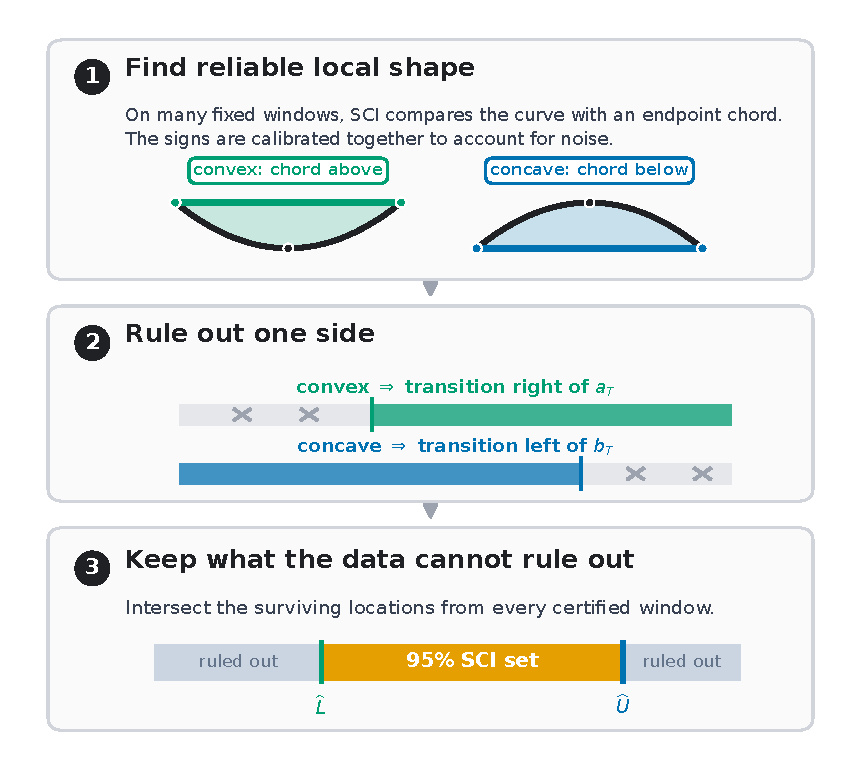
\includegraphics[width=0.88\linewidth]{figures/sci_method_overview.pdf}
\caption{A plain-language overview of \SCI.  (1) Endpoint chords provide local
evidence for convexity or concavity; the implementation averages these
residuals and calibrates all fixed windows together.  (2) Certified convexity
rules out transition locations on the left, while certified concavity rules
out locations on the right.  (3) Intersecting all surviving locations gives
the \SCI confidence set.  This schematic illustrates the inversion logic; it
is not a substitute for the coverage proof.}
\label{fig:sci-method}
\end{figure}
\FloatBarrier

\section{Finite-sample theory}
\label{sec:theory}

\begin{theorem}[Known-scale finite-sample coverage]
\label{thm:known}
Suppose $\varepsilon_i\stackrel{\mathrm{iid}}{\sim}N(0,\sigma^2)$, the finite
contrast family $\T$ is fixed independently of $Y$, and every row has the sign
property stated above.  Then, uniformly over every $f$ with
$\I(f)\neq\varnothing$,
\[
  \Ph_f\{\I(f)\subseteq\widehat\C(Y)\}\geq1-\alpha.
\]
Consequently,
$\Ph_f\{\widehat\C(Y)=\varnothing\}\leq\alpha$ whenever the target is
nonempty.
\end{theorem}

The theorem is exact for the stated Gaussian model.  It is not an asymptotic
bootstrap result.  It covers all compatible locations at once and therefore
remains meaningful when the target is an interval.

\begin{proposition}[Minimal interval from the certified signs]
\label{prop:minimal}
Condition on the collection of certified positive and negative signs.  Among
closed intervals that use only those logical sign implications,
$[\widehat L,\widehat U]$ is the smallest one containing every transition that
has not been excluded.
\end{proposition}

Proposition~\ref{prop:minimal} is a logical minimality result.  It does not say
that \SCI is the shortest possible confidence procedure.  A different joint
band or additional model assumptions can give a smaller set.

\subsection{Localization under a contrast margin}

Coverage alone does not ensure that the set is informative.  The next result
states the signal strength needed for localization.  It also makes clear why
weak smooth transitions can produce wide sets.

\begin{assumption}[Contrast margin at scale $d$]
\label{ass:margin}
Write $\I(f)=[m_-,m_+]$.  For a scale $d>0$, suppose the family contains
\begin{enumerate}[label=(\roman*),leftmargin=*]
  \item a left contrast $T_-$ with
  $a_{T_-}\geq m_- - Kd$, $\mu_{T_-}\geq Bd^\gamma$, and
  $\norm{w_{T_-}}\leq C_w/\sqrt{nd}$; and
  \item a right contrast $T_+$ with
  $b_{T_+}\leq m_+ + Kd$, $\mu_{T_+}\leq-Bd^\gamma$, and
  $\norm{w_{T_+}}\leq C_w/\sqrt{nd}$.
\end{enumerate}
Here $B,C_w,K>0$ and $\gamma>0$ do not depend on $n$.
\end{assumption}

\begin{theorem}[Margin-based localization]
\label{thm:margin}
Under Theorem~\ref{thm:known} and
Assumption~\ref{ass:margin}, let $0<\eta<1$ and suppose
\begin{equation}
  Bd^\gamma\geq
  \frac{\sigma C_w}{\sqrt{nd}}
  \left(c_{\alpha,M}+z_{1-\eta/2}\right),
\label{eq:margincondition}
\end{equation}
where $z_q=\Phi^{-1}(q)$.  Then, with probability at least
$1-\alpha-\eta$,
\[
  \I(f)\subseteq\widehat\C(Y)
  \subseteq[m_- - Kd,m_+ + Kd].
\]
In particular,
$|\widehat\C(Y)|\leq|\I(f)|+2Kd$ on this event.
\end{theorem}

Balancing the two sides of \eqref{eq:margincondition} gives the detection scale
\begin{equation}
 d_n\asymp
 \left\{\frac{\sigma^2(c_{\alpha,M}+z_{1-\eta/2})^2}
 {B^2n}\right\}^{1/(2\gamma+1)}.
\label{eq:generalrate}
\end{equation}
When $M$ grows polynomially with $n$, $c_{\alpha,M}^2=O(\log n)$, so the
excess length is conditionally
$O_{\Ph}\{(\sigma^2\log n/(B^2n))^{1/(2\gamma+1)}\}$.
This statement is conditional on the explicit margin and contrast availability.
It is not yet a broad minimax theorem for every S-shaped function class.

\subsection{Cubic transition}

The standard smooth reference case is a cubic crossing.  Let
$x_i=i/(n+1)$ and
\[
  f(x)=c_0+c_1(x-m_0)-B(x-m_0)^3,
  \qquad B>0.
\]
For the dyadic contrast family in Appendix~\ref{app:contrasts}, define
\begin{equation}
  h_*=\left\{
  \frac{\sigma(c_{\alpha,M_n}+z_{1-\eta/2})}
  {\sqrt{6}B\sqrt{n+1}}
  \right\}^{2/7}.
\label{eq:hstar}
\end{equation}

\begin{corollary}[Exact cubic localization order]
\label{cor:cubic}
Put $q_*=(n+1)h_*$, assume $q_*\geq1$, and let $q$ be the smallest dyadic
integer with $q\geq q_*$.  If $3q\leq n$ and
$m_0\in[8h_*,1-8h_*]$, then
\[
  \Ph_f\{m_0\in\widehat\C(Y),\ |
  \widehat\C(Y)|<16h_*\}\geq1-\alpha-\eta.
\]
Thus
\[
 |\widehat\C(Y)|=
 O_{\Ph}\!\left\{
 \left(\frac{\sigma^2\log n}{B^2n}\right)^{1/7}
 \right\}.
\]
\end{corollary}

For the three frozen separation multipliers,
$M_n\leq6n+6(1+\log_2 n)$.  Hence the polynomial-size condition used for the
displayed stochastic order holds directly.

The $n^{-1/7}$ power is the known regular order for localizing a root of a
second derivative.  Related orders appear in
\citet{schmidthieber2013multiscale} and \citet{feng2022sshaped}.  The value of
Corollary~\ref{cor:cubic} is compatibility: \SCI keeps finite-sample validity
over a wider nonsmooth class without losing this reference order in the cubic
case.

\section{Unknown and nonconstant noise}
\label{sec:extensions}

The inversion only needs simultaneous bounds for the contrast means.  This
modularity gives three useful extensions.

\subsection{Unknown constant scale}

Let $X\in\R^{n\times r}$ be a fixed full-rank nuisance design and let
$R_X=I-P_X$ be its residual projector.  Write
$q_{\nu,\eta}$ for the lower $\eta$ quantile of a chi-squared random variable
with $\nu$ degrees of freedom, and define
\begin{equation}
  \overline\sigma=
  \left\{\frac{\norm{R_XY}^2}{q_{n-r,\eta}}\right\}^{1/2}.
\label{eq:sigmabar}
\end{equation}

\begin{theorem}[Honest upper scale bound]
\label{thm:unknown}
If $Y=\mu+\varepsilon$ with arbitrary deterministic $\mu\in\R^n$ and
$\varepsilon\sim N(0,\sigma^2I)$, then
\[
  \inf_{\mu,\sigma>0}\Ph_{\mu,\sigma}
  (\overline\sigma\geq\sigma)\geq1-\eta.
\]
If \eqref{eq:band} uses $\overline\sigma$ and error budget
$\alpha-\eta$, the resulting \SCI set covers $\I(f)$ with probability at
least $1-\alpha$.
\end{theorem}

No independence between the scale estimate and the contrasts is required.
The price is conservatism: the residual norm can contain unremoved signal.
Our default nuisance space uses fixed blocks of size two.  For sampled monotone
curves with bounded total variation, its signal contribution becomes negligible
in the usual increasing-design limit.

\subsection{Bounded heteroskedasticity}

Now let the errors be independent with
$\varepsilon_i\sim N(0,\sigma_i^2)$.  A finite-sample result requires some
information about the unobserved variance pattern.  We make that information
explicit.

\begin{assumption}[Variance-ratio bound]
\label{ass:kappa}
For a declared $\kappa\geq1$,
\[
  \max_i\sigma_i^2\leq\kappa\bar\sigma^2,
  \qquad
  \bar\sigma^2=\frac1n\sum_{i=1}^n\sigma_i^2.
\]
\end{assumption}

Use a fixed partition into blocks of size two or three, and let $R$ remove the
constant within each block.  Set $Q=\norm{RY}^2$ and
\begin{align}
 d_{n,\kappa,\eta}
   &=1-2\sqrt{\frac{2\kappa\log(1/\eta)}{n}},
   \label{eq:dnk}\\
 \widehat\sigma_{\max}^2
   &=\frac{2\kappa Q}{n d_{n,\kappa,\eta}}.
   \label{eq:sigmamax}
\end{align}

\begin{theorem}[Heteroskedastic scale envelope]
\label{thm:hetero}
Under Assumption~\ref{ass:kappa}, if $d_{n,\kappa,\eta}>0$, then
\[
  \Ph\left(\widehat\sigma_{\max}^2
  \geq\max_i\sigma_i^2\right)\geq1-\eta
\]
uniformly over the mean vector and all variance vectors satisfying the
assumption.  Replacing each contrast standard error by
$\widehat\sigma_{\max}\norm{w_T}$ and using error budget $\alpha-\eta$
therefore gives at least $1-\alpha$ coverage.
\end{theorem}

The proof uses Anderson's inequality for a translated Gaussian norm
\citep{anderson1955integral} and a weighted chi-squared lower-tail inequality
\citep{laurent2000adaptive}.  The method is a sensitivity analysis: its claim
is only as credible as the chosen $\kappa$.  Larger values correctly give wider
sets.

\subsection{Independent replicate curves}

Suppose we observe $R$ independent curves
\[
  Y_r\sim N(\mu,\Sigma),\qquad r=1,\ldots,R,
\]
where the common covariance $\Sigma$ may be non-diagonal or singular.  For a
contrast row $w_j$, let $Z_{rj}=w_j^\top Y_r$, with sample mean
$\bar Z_j$ and sample standard deviation $s_j$ across replicates.

\begin{theorem}[Replicate Student band]
\label{thm:replicate}
For $M$ fixed contrasts, the intervals
\[
  \bar Z_j\ \pm\ t_{R-1,1-\alpha/(2M)}\frac{s_j}{\sqrt R},
  \qquad j=1,\ldots,M,
\]
cover all contrast means simultaneously with probability at least $1-\alpha$.
Their sign inversion therefore satisfies
$\Ph\{\I(\mu)\subseteq\widehat\C\}\geq1-\alpha$.
\end{theorem}

Dependence and unequal variance across design locations are allowed inside one
replicate.  Independence is required across replicates, which is the correct
sampling unit in repeated-curve studies \citep{davidian1995nonlinear}.

\section{Computation and matched honest baseline}
\label{sec:computation}

\subsection{Matrix-free implementation}

Writing all contrast rows as an $M\times n$ matrix is unnecessary.  On a
uniform design, block averages and chord residuals can be evaluated from prefix
sums.  The implementation stores only scale metadata and start indices.  The
default separation family uses ratios $(1,2,4)$ across dyadic scales.

Table~\ref{tab:scaling} gives a deterministic scaling benchmark.  Times are
hardware-specific, while storage and dense counterfactual sizes follow directly
from the constructed family.  At $n=10^6$, the implementation evaluates
5,999,750 contrasts in 0.73 seconds and stores 53.4 MiB.  A dense double matrix
would require about 44,702 GiB.

\begin{table}[htbp]
\centering
\caption{Matrix-free scaling for the full $(1,2,4)$ separation family.}
\label{tab:scaling}
\small
\begin{tabular}{rrrrrr}
\toprule
$n$ & Contrasts & Build (s) & Evaluate (s) & Stored (MiB) & Dense (GiB)\\
\midrule
1,000     & 5,872     & 0.0006 & 0.0015 & 0.05 & 0.04\\
10,000    & 59,831    & 0.0009 & 0.0039 & 0.53 & 4.46\\
100,000   & 599,790   & 0.0042 & 0.0287 & 5.34 & 446.88\\
1,000,000 & 5,999,750 & 0.0346 & 0.7318 & 53.40 & 44,701.62\\
\bottomrule
\end{tabular}
\end{table}

\subsection{Pointwise-band projection}

To compare two methods with the same type of guarantee, we construct a generic
pointwise confidence box
\[
  \mathcal B(Y)=\prod_{i=1}^n
  [Y_i-z_{1-\alpha/(2n)}\sigma,
   Y_i+z_{1-\alpha/(2n)}\sigma].
\]
For each possible cut, a linear program asks whether this box contains a vector
that is discretely convex before the cut and concave after it.  The outer range
of feasible cuts is \PBP.  If the complete mean vector lies in the box, every
true cut is feasible.  Bonferroni therefore gives the same finite-sample
coverage target as \SCI.  \PBP spends error probability on every coordinate;
\SCI spends it on the feature-specific contrasts.  The comparison measures the
gain from targeting the scientific feature directly.

\section{Simulation experiments}
\label{sec:experiments}

\subsection{Design}

We use four benchmark signals from the S-shaped estimation study of
\citet{feng2022sshaped}: a cusp, a one-sided onset, a jump, and a smooth logistic
curve.  The first three stress nonsmooth behavior; the logistic signal is the
smooth reference case.  Designs are either uniform or sampled from a
$\operatorname{Beta}(4,8)$ distribution.  Sample sizes are $n=500$ and
$n=1000$, the Gaussian standard deviation is $0.1$, and the nominal confidence
level is 95\%.

The study was staged.  An initial comparison used 200 responses per cell and
included the S-shaped least-squares point estimator (\texttt{Sshaped} 1.2) and
the residual-bootstrap interval from \texttt{ShapeChange} 1.5 with 1,000
bootstrap samples.  We then froze the \SCI configuration and ran a fresh
high-precision audit with 5,000 responses in each of 16 cells, or 80,000
responses in total.  Finally, a separate 200-response-per-cell experiment
compared \SCI with the matched honest \PBP baseline.  Failures and empty sets
were never discarded.

\subsection{High-precision coverage audit}

Table~\ref{tab:e36} summarizes the 80,000-response audit.  Coverage is stable
between 0.9770 and 0.9804.  The simultaneous contrast band itself covers all
contrast means in 0.9524--0.9618 of responses, close to the intended 0.95
familywise level.  The larger transition-set coverage is expected because not
every missed contrast bound changes the inverted set.

\begin{table}[htbp]
\centering
\caption{High-precision known-scale audit.  Each row summarizes four fixed
design--sample-size cells with 5,000 responses per cell.}
\label{tab:e36}
\small
\begin{tabular}{lccc}
\toprule
Signal & Coverage range & Median-width range & Largest empty rate\\
\midrule
Cusp     & 0.9772--0.9804 & 0.0712--0.1737 & 0.0182\\
Onset    & 0.9772--0.9788 & 0.6703--0.8149 & 0.0066\\
Jump     & 0.9770--0.9798 & 0.0020--0.0100 & 0.0228\\
Logistic & 0.9776--0.9798 & 0.9990--1.0000 & 0.0006\\
\bottomrule
\end{tabular}
\end{table}

The widths contain the main scientific message.  The jump is localized very
sharply, the cusp moderately, and the one-sided onset only partly.  The weak
logistic curvature does not produce reliable local signs, so the answer is
almost the whole design range.  This is not a computational failure.  It is the
honest statement that the chosen data and noise level do not identify the
transition precisely.

One preregistered diagnostic required zero empty sets.  It failed: empty-set
frequencies reached 2.28\%.  Theorem~\ref{thm:known} only requires this
probability to be at most 5\% for a nonempty target, and the Wilson upper bounds
remain below 5\% in all cells.  We nevertheless report the frozen diagnostic as
failed rather than redefining it after seeing the results.

\subsection{Published comparator and hybrid workflow}

Figure~\ref{fig:e33} shows the initial comparison.  \SCI coverage was
0.965--0.995.  The \texttt{ShapeChange} residual-bootstrap interval had zero
coverage in 9 of 16 cells, all involving nonsmooth signals outside its
documented smooth spline regime.  In the four smooth logistic cells its
coverage was 0.960--0.990 and its intervals were narrower.  The correct use is
therefore a hybrid: retain a strong S-shaped estimator as the point summary,
and use \SCI when the uncertainty claim must remain valid under nonsmoothness.

The hybrid did not improve point-estimation error.  Aggregated mean absolute
error was 0.06236 for the published S-shaped estimator and 0.06276 after a
simple projection.  We therefore make no ``point-estimator booster'' claim.
The value of \SCI is calibrated uncertainty around the point estimate.

\begin{figure}[htbp]
\centering
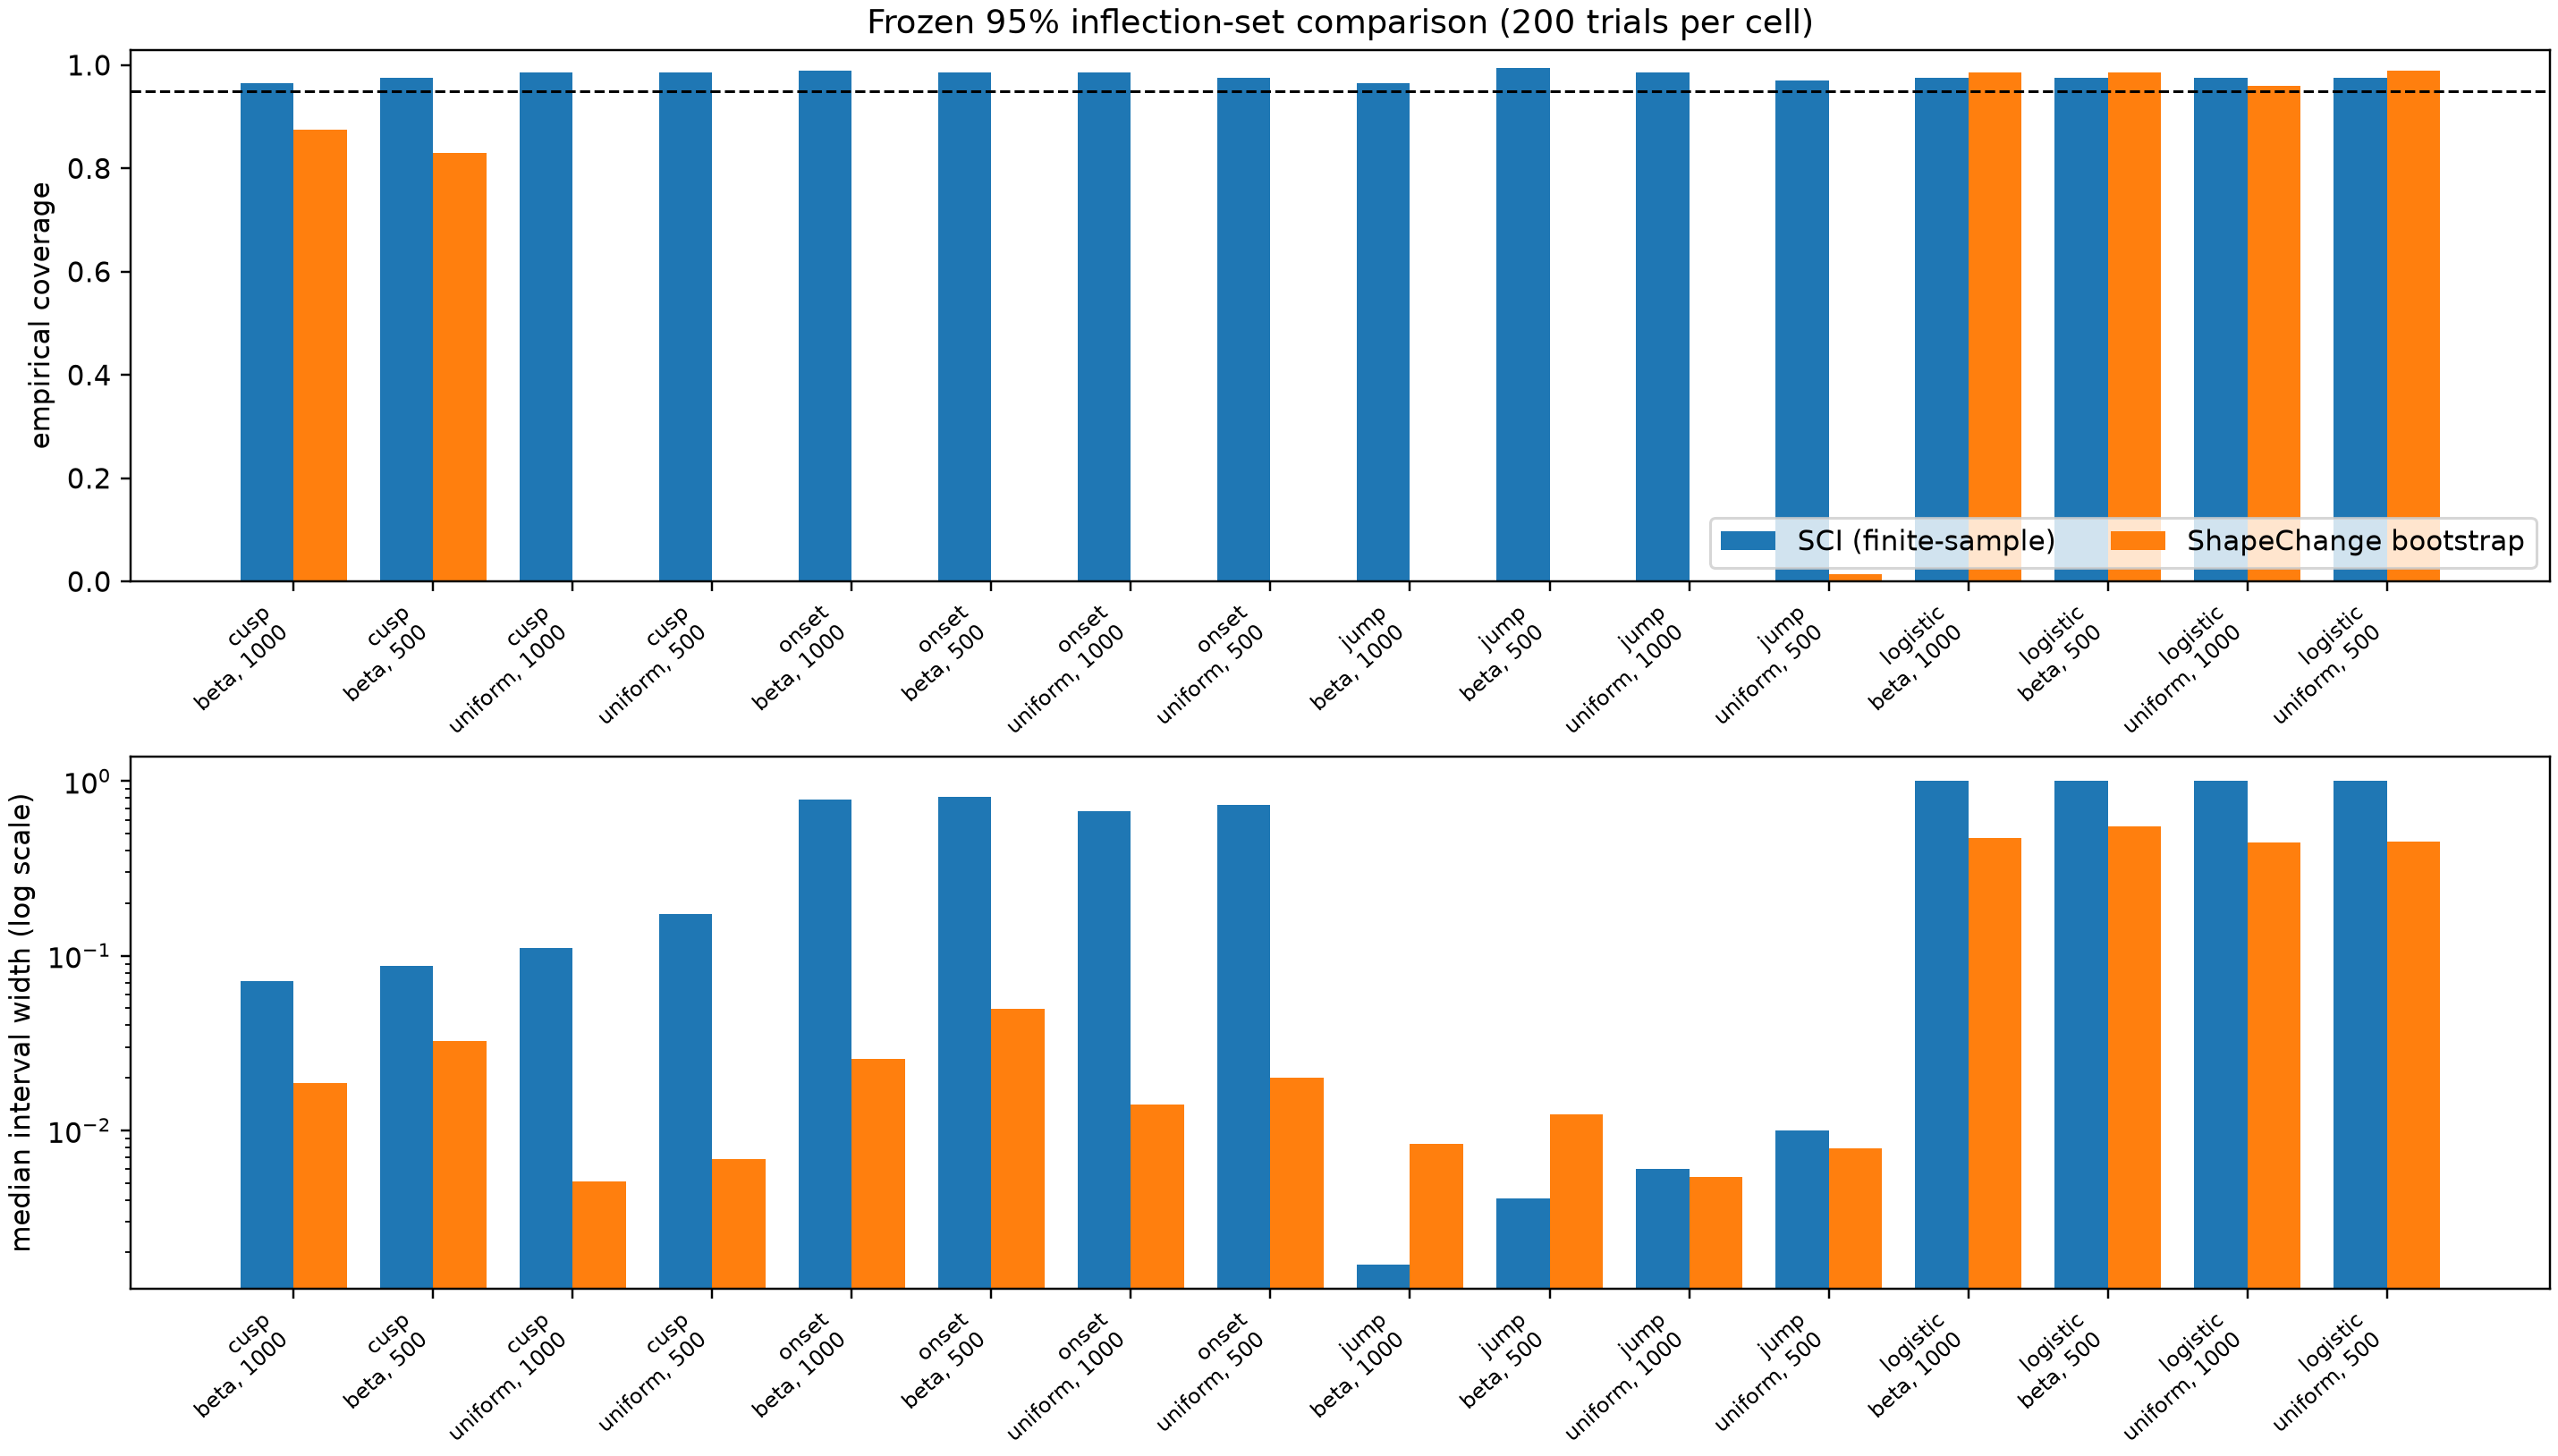
\includegraphics[width=0.96\linewidth]{figures/e33_frontier_coverage_width.png}
\caption{Coverage and width in the initial comparison.  The smooth-bootstrap
comparator is used inside and outside its smooth regime to expose the practical
robustness gap; the comparison does not contradict its published assumptions.}
\label{fig:e33}
\end{figure}

\subsection{Matched honest comparison}

Table~\ref{tab:e38} compares \SCI and \PBP under the same Gaussian model and
nominal coverage target.  Both methods covered in every cell at the expected
or conservative rate.  For the cusp, onset, and jump, \SCI reduced median width
by 19.4\%--75.7\%.  For the weak logistic signal, both methods returned the same
nearly full range.  This experiment isolates the useful gain: direct
feature-specific inversion can be much sharper than projecting a generic
confidence box, but it cannot manufacture information when curvature is too
weak.

\begin{table}[htbp]
\centering
\caption{Matched honest comparison with 200 responses per cell.  ``Beta'' is
the $\operatorname{Beta}(4,8)$ design.  Reduction is relative median width.}
\label{tab:e38}
\scriptsize
\setlength{\tabcolsep}{4.2pt}
\begin{tabular}{llrrrrrr}
\toprule
Signal & Design & $n$ & \SCI\ cov. & \PBP\ cov. & \SCI\ width & \PBP\ width & Reduction\\
\midrule
Cusp & Uniform & 500  & .985 & 1.000 & .1737 & .4122 & 57.9\%\\
Cusp & Uniform & 1000 & .965 & 1.000 & .1109 & .3861 & 71.3\%\\
Cusp & Beta    & 500  & .950 & 1.000 & .0877 & .3151 & 72.2\%\\
Cusp & Beta    & 1000 & .995 & 1.000 & .0712 & .2934 & 75.7\%\\
Onset & Uniform & 500  & .975 & .995 & .7325 & .9960 & 26.5\%\\
Onset & Uniform & 1000 & .980 & 1.000 & .6703 & .9980 & 32.8\%\\
Onset & Beta    & 500  & .980 & 1.000 & .5460 & .6776 & 19.4\%\\
Onset & Beta    & 1000 & .985 & 1.000 & .5170 & .7116 & 27.3\%\\
Jump & Uniform & 500  & .965 & 1.000 & .0100 & .0180 & 44.4\%\\
Jump & Uniform & 1000 & .980 & .995 & .0050 & .0090 & 44.4\%\\
Jump & Beta    & 500  & .975 & .995 & .0041 & .0068 & 40.0\%\\
Jump & Beta    & 1000 & .985 & 1.000 & .0017 & .0034 & 50.0\%\\
Logistic & Uniform & 500  & .970 & 1.000 & .9960 & .9960 & 0.0\%\\
Logistic & Uniform & 1000 & .965 & 1.000 & .9980 & .9980 & 0.0\%\\
Logistic & Beta    & 500  & .975 & 1.000 & .6776 & .6776 & 0.0\%\\
Logistic & Beta    & 1000 & .975 & 1.000 & .7116 & .7116 & 0.0\%\\
\bottomrule
\end{tabular}
\end{table}

For this matched experiment, both procedures were restricted to the observed
design range $[x_1,x_n]$.  This matters for the random Beta design: its observed
range is shorter than $[0,1]$.  The high-precision audit in
Table~\ref{tab:e36} instead used the full scientific domain $[0,1]$.

\subsection{Unknown-scale and heteroskedastic checks}

The unknown-homoskedastic experiment contained 28 frozen cells.  The minimum
\SCI coverage was 0.990, the minimum coverage of the upper scale bound was
0.975, and the mean width inflation among informative cells was 1.117 relative
to known scale.  All frozen gates passed.

The bounded-heteroskedastic experiment contained 48 cells spanning constant,
linear, and plume-like variance profiles.  The minimum transition coverage and
the minimum scale-envelope coverage were both 0.995.  These results test the
implementation of Theorems~\ref{thm:unknown} and~\ref{thm:hetero}; the guarantees
themselves come from the theorems, not from Monte Carlo performance.

\section{Real-data illustrations}
\label{sec:data}

\subsection{Atmospheric LIDAR}

The LIDAR example studies a response curve over altitude.  A published
S-shaped point fit places the transition at 588 m.  The
\texttt{ShapeChange} fit gives 606 m with a residual-bootstrap interval
$[592.6,612.8]$ m.  Visible variance changes make that iid-bootstrap interval
descriptive here.

Figure~\ref{fig:lidar} reports the \SCI sensitivity analysis.  With
$\kappa=1$, the set is $[510,664]$ m.  It grows to $[486,720]$ m for
$\kappa=1.5$, $[438,720]$ m for $\kappa=2$, and $[390,720]$ m for
$\kappa\geq3$ in the displayed range.  The conclusion is conditional: if the
maximum variance is at most $\kappa$ times the mean variance, the corresponding
set has the finite-sample guarantee.  The widening shows the cost of making a
more cautious variance claim.

\begin{figure}[htbp]
\centering
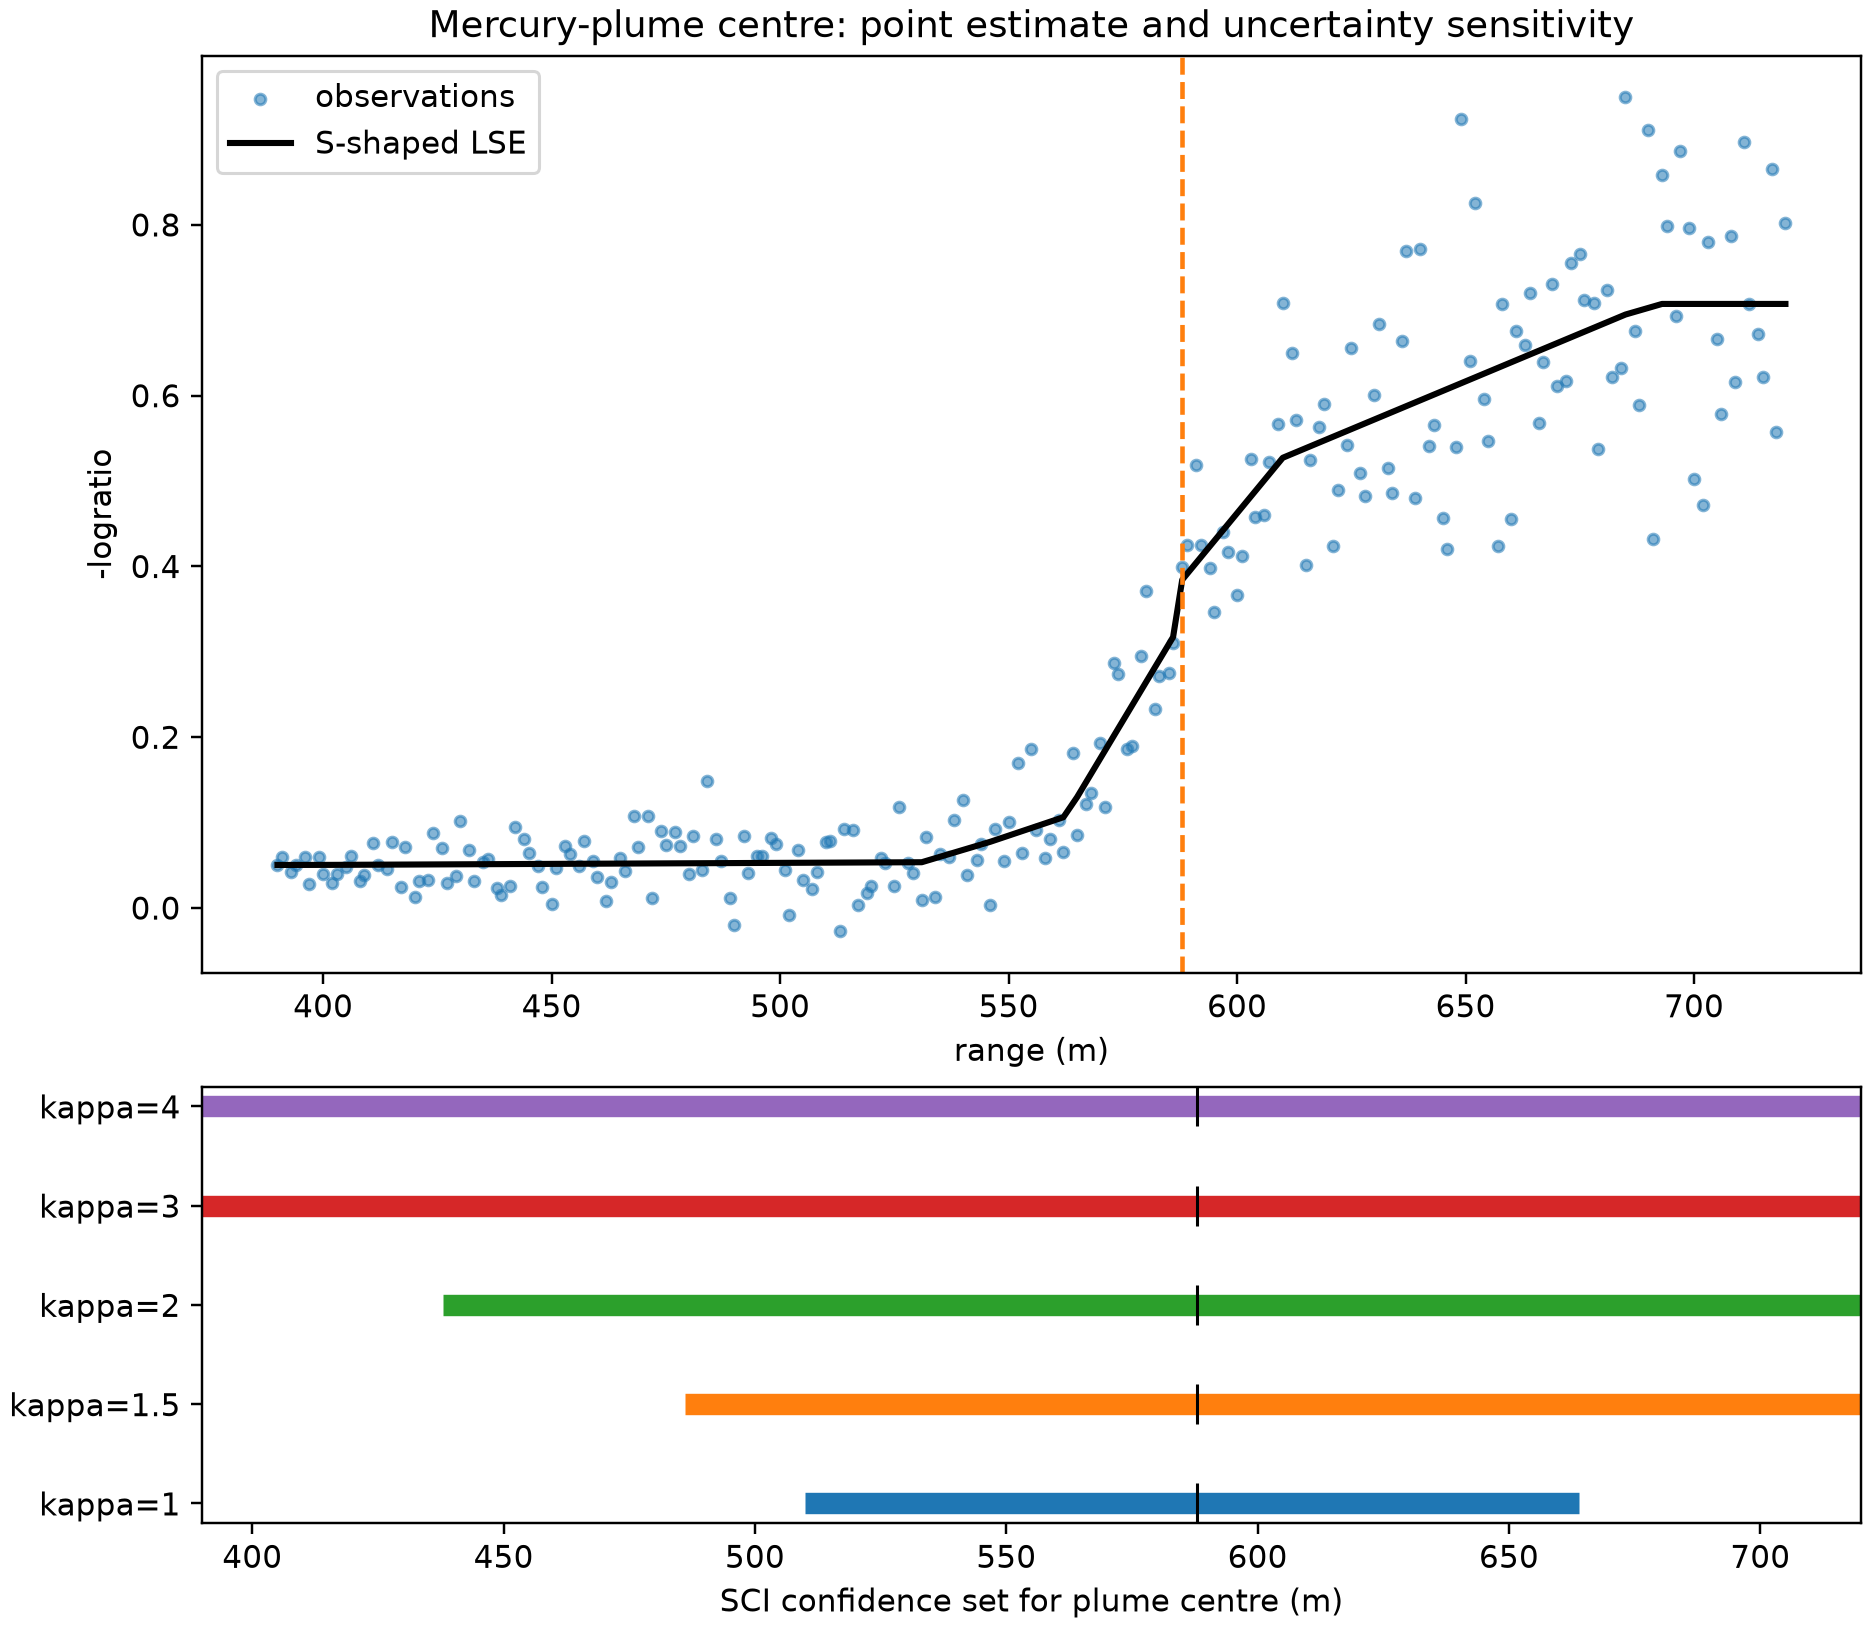
\includegraphics[width=0.88\linewidth]{figures/lidar_sci_sensitivity.png}
\caption{LIDAR transition sets under the declared variance-ratio bound
$\kappa$.  Larger heterogeneity allowances produce wider honest sets.}
\label{fig:lidar}
\end{figure}

\subsection{Replicated DNase assay}

The DNase data distributed with R contain 11 assay runs and eight
concentrations \citep{r2025}.  We use all 176 raw optical-density measurements.
Technical duplicates are averaged within each run, and the run is the
independent unit.  This leaves 11 replicate curves on the same eight-point
design.

The replicate Student construction gives the 95\% transition set
$[0.78125,12.5]$ in concentration units.  A four-parameter logistic fit gives
the descriptive midpoint 4.1412.  The point lies inside the confidence set,
but the set reaches the largest observed concentration.  The data support a
lower limit, while they do not supply a reliable upper limit inside the
observed range.

The exact statement assumes independent Gaussian replicate curves with a
common mean and covariance.  With only 11 runs, the interval is necessarily
conservative.  Treating all 176 readings as independent would give a narrower
but invalid answer because technical duplicates and concentrations from the
same run are correlated.

\begin{figure}[htbp]
\centering
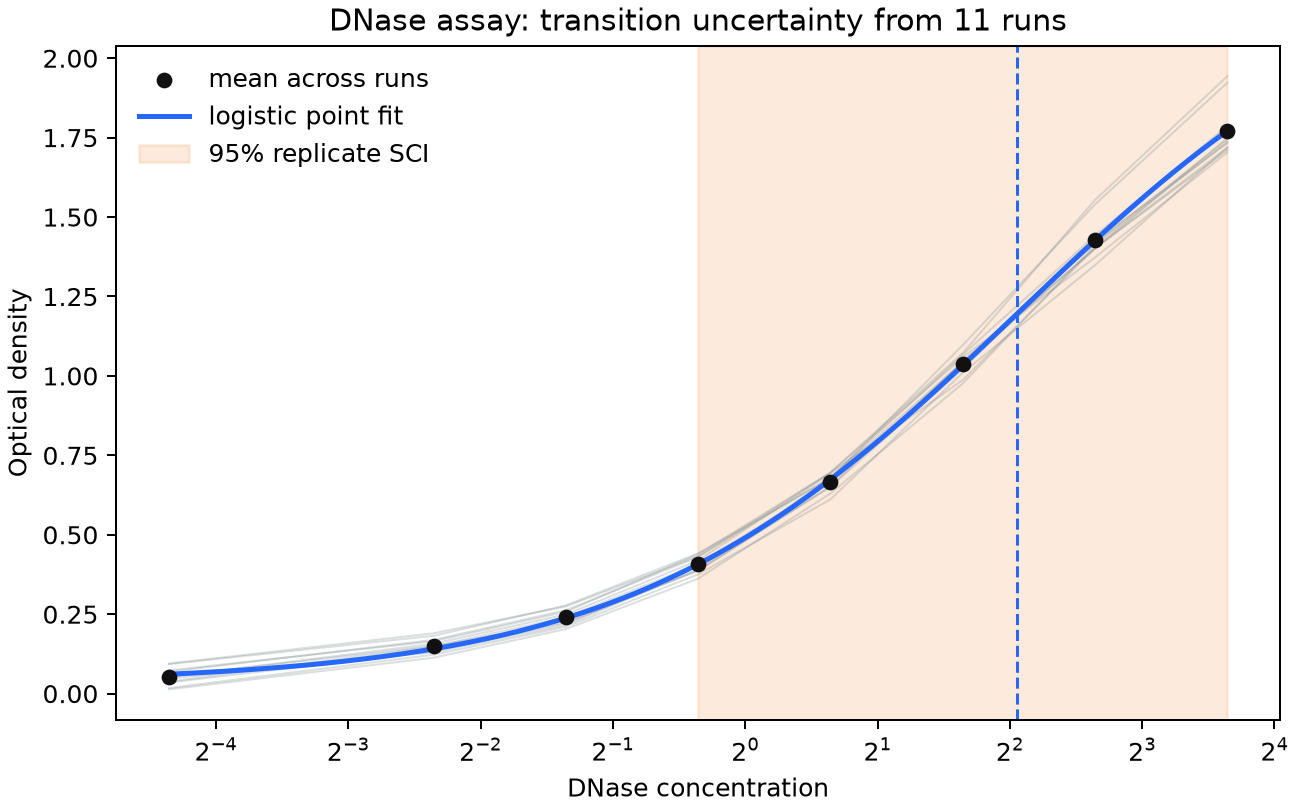
\includegraphics[width=0.85\linewidth]{figures/dnase_replicate_sci.png}
\caption{DNase run means, replicate mean curve, descriptive logistic midpoint,
and the 95\% replicate-curve \SCI set.  Dependence across concentrations inside
a run is allowed.}
\label{fig:dnase}
\end{figure}

\section{Discussion}
\label{sec:discussion}

\subsection{What practical problem is solved?}

The method solves a specific uncertainty problem: it gives a finite-sample
outer confidence set for every convex-to-concave transition that is compatible
with a sampled mean curve, without assuming a smooth or unique inflection.  A
researcher can attach this set to an S-shaped point estimate and distinguish
three outcomes:
\begin{enumerate}[leftmargin=*]
  \item a narrow set, meaning that the data certify local shape signs close to
  the fitted transition;
  \item a one-sided or wide set, meaning that only part of the location is
  identified; and
  \item an empty set, which is a controlled rare event under the model but can
  also flag model tension in practice.
\end{enumerate}

This addresses the gap exposed by the experiments.  A smooth bootstrap can be
sharp when its assumptions hold but fail badly on nonsmooth signals.  A generic
honest confidence region remains valid but can be unnecessarily wide.  \SCI
keeps the broad nonsmooth guarantee while using feature-specific evidence to
improve width in informative cases.

\subsection{What is not claimed?}

First, \SCI is not a new point estimator and did not improve point-estimation
error in our hybrid experiment.  Second, it is not the first inference method
for inflection points.  Third, the $(\log n/n)^{1/7}$ cubic rate is not new.
Fourth, the output is an outer set, not a proof that every included point is a
true physical threshold.  Finally, the real-data conclusions are conditional
on their sampling models.

\subsection{Limitations and open work}

The exact single-curve results are Gaussian.  A self-normalized or
distribution-robust band would broaden the method.  The heteroskedastic
extension needs a user-declared $\kappa$; it cannot learn an unrestricted
variance vector from one observation per design point.  The replicate result
needs independent runs with a common covariance.  Bonferroni calibration is
simple and transparent but can be conservative when many contrasts overlap.

The main theoretical gap is also clear.  Theorem~\ref{thm:margin} gives a rate
under explicit contrast-margin and availability conditions.  A broad
function-class lemma that derives these conditions automatically, together
with a matching lower bound for the set-valued target, remains open.  Such a
result could turn the current conditional rate into a minimax characterization.

\section{Conclusion}

Shape-contrast inversion turns local geometric evidence into an honest
uncertainty statement for a convex-to-concave transition.  Its main strength is
not a universally narrow interval.  It is the combination of finite-sample
coverage, tolerance of nonsmooth and nonunique transitions, and a direct
matrix-free implementation.  The matched comparison shows that targeting the
feature can be much sharper than projecting a generic confidence box.  The
logistic and DNase examples show the equally important other side: when the
data do not support precise localization, the method says so.

\section*{Reproducibility statement}

The public repository contains the matrix-free implementation, frozen
experiment configurations, raw trial-level outputs, summaries, figures, and
verification manifests.  All reported numerical claims are generated from
these artifacts.  The release test suite contains 228 tests, including 48
specific to \SCI.  The release manifest verifies 1,565 files, and the SCI
artifact verifier checks 60 frozen SCI files.  Commands for rebuilding this
manuscript are given beside the source.

\section*{CRediT authorship contribution statement}

Saveliy Baturin: Conceptualization; Methodology; Software; Validation; Formal
analysis; Investigation; Data curation; Visualization; Writing -- original
draft; Writing -- review and editing.

\section*{Declaration of competing interest}

The author declares no competing financial interests or personal
relationships that could have appeared to influence the work reported here.

\section*{AI assistance disclosure}

The author used OpenAI Codex to assist with literature organization, software
engineering, verification, and language editing.  The mathematical claims,
experimental design, reported results, and final interpretations were checked
and approved by the author, who assumes full responsibility for the manuscript.

\appendix

\section{Contrast construction}
\label{app:contrasts}

The implementation uses a fixed dyadic family.  For a scale $q$, a start index
$s$, and separation multiplier $g\in\{1,2,4\}$, it selects left, middle, and
right blocks of comparable size with separation $gq$.  Each block chord
residual is a nonnegative average of elementary terms of the form
\eqref{eq:chord}.  The exact weights account for irregular design spacing.
Their sum is zero, so affine functions have zero contrast.  Convex functions
give a nonnegative mean and concave functions a nonpositive mean.

The family includes all admissible starts at each dyadic scale.  It is fixed
from the design before the responses are read.  On a uniform design, prefix
sums of $Y_i$ and $iY_i$ evaluate each block average in constant time.  The
known-scale standard error is computed from the closed-form squared norm of the
stored row.  Irregular designs use sparse index and weight arrays rather than a
dense $M\times n$ matrix.

\section{Proofs}
\label{app:proofs}

\begin{proof}[Proof of Lemma~\ref{lem:identified}]
Because $m_2\in\I(f)$, the function is convex on $[A,m_2]$, hence on
$[m_1,m_2]$.  Because $m_1\in\I(f)$, it is concave on $[m_1,B]$, hence on the
same interval.  A real-valued function that is both convex and concave on an
interval is affine there.  For any $m\in[m_1,m_2]$, membership of $m_2$ gives
convexity on $[A,m]$, while membership of $m_1$ gives concavity on $[m,B]$.
Thus $m\in\I(f)$.
\end{proof}

\begin{proof}[Proof of Theorem~\ref{thm:known}]
For each $T$, $Z_T-\mu_T$ is centered normal with standard deviation
$\sigma\norm{w_T}$.  By \eqref{eq:critical} and a union bound,
\[
  \Ph\{\ell_T\leq\mu_T\leq u_T\text{ for all }T\in\T\}
  \geq1-\alpha.
\]
Call this event $E$ and fix $m\in\I(f)$.  If $\ell_T>0$ and
$a_T\geq m$, the support lies in the concave part of $f$, so
$\mu_T\leq0$.  This contradicts $\ell_T\leq\mu_T$ on $E$.  Therefore every
certified positive contrast has $a_T<m$, and $\widehat L\leq m$.  Likewise,
if $u_T<0$ and $b_T\leq m$, the support lies in the convex part, so
$\mu_T\geq0$, contradicting $\mu_T\leq u_T$.  Hence $m\leq\widehat U$.
The argument holds for every $m\in\I(f)$ on the same event $E$, so
$\I(f)\subseteq[\widehat L,\widehat U]=\widehat\C(Y)$.  The uniform bound
follows because the probability of $E$ does not depend on $f$.
\end{proof}

\begin{proof}[Proof of Proposition~\ref{prop:minimal}]
A certified positive contrast rules out only points at or below its left
endpoint by the stated sign logic.  Combining all such statements gives the
largest lower limit $\widehat L$.  A certified negative contrast rules out only
points at or above its right endpoint, giving the smallest upper limit
$\widehat U$.  Thus every point in $[\widehat L,\widehat U]$ survives all
certified implications, while every point outside violates at least one of
them.  Any closed interval based only on these implications and containing all
surviving points must contain $[\widehat L,\widehat U]$.
\end{proof}

\begin{proof}[Proof of Theorem~\ref{thm:margin}]
The simultaneous band event from Theorem~\ref{thm:known} has probability at
least $1-\alpha$.  Separately,
\[
  \Ph\left\{Z_{T_-}>
  \mu_{T_-}-z_{1-\eta/2}\sigma\norm{w_{T_-}}\right\}
  \geq1-\eta/2,
\]
and the analogous upper-tail statement holds for $T_+$.  A union bound gives
all three events with probability at least $1-\alpha-\eta$.
Condition \eqref{eq:margincondition} then implies $\ell_{T_-}>0$ and
$u_{T_+}<0$.  Therefore
$\widehat L\geq a_{T_-}\geq m_- - Kd$ and
$\widehat U\leq b_{T_+}\leq m_+ + Kd$.  The simultaneous band event also gives
$\I(f)\subseteq\widehat\C(Y)$ by Theorem~\ref{thm:known}.  The length bound
follows.
\end{proof}

\begin{proof}[Proof of Corollary~\ref{cor:cubic}]
For a symmetric equally spaced triple with middle location $u$ and physical
separation $d$, direct expansion of the cubic gives
\begin{equation}
  Q(f)=3B(m_0-u)d^2.
\label{eq:cubicq}
\end{equation}
Take an implemented multiplier-one row of block size $q$.  Its $q$ triples
have physical separation $d=q/(n+1)$ and use disjoint left, middle, and right
blocks.  Its coefficient norm is therefore exactly
\begin{equation}
  \norm{w_T}=\sqrt{\frac{3}{2q}}.
\label{eq:cubicnorm}
\end{equation}

Choose the rightmost allowed start, on the $q$-spaced grid of starts, whose
whole support ends at or before $m_0$.  The interior condition ensures that it
exists.  Every triple has its right point at or before $m_0$, so its middle
point is at least $d$ to the left of $m_0$.  Equation~\eqref{eq:cubicq} gives
$\mu_T\geq3Bd^3$.  Maximality of the start also puts its support beginning less
than $4d$ to the left of $m_0$.  With \eqref{eq:cubicnorm},
\[
  \frac{\mu_T}{\sigma\norm{w_T}}
  \geq\frac{\sqrt6B\sqrt{n+1}\,d^{7/2}}{\sigma}
  \geq c_{\alpha,M_n}+z_{1-\eta/2},
\]
where the last step uses $q\geq q_*$.  This row fails to be certified positive
with probability at most $\eta/2$.

The symmetric construction uses the leftmost $q$-grid start whose support
begins at or after $m_0$.  It gives a negative row with failure probability at
most $\eta/2$ and support ending less than $4d$ to the right of $m_0$.
When both rows are certified,
$\widehat L>m_0-4d$ and $\widehat U<m_0+4d$.  The smallest-dyadic choice gives
$q<2q_*$, so $d<2h_*$ and
$\widehat U-\widehat L<16h_*$.  Intersecting with the simultaneous-band event
of Theorem~\ref{thm:known} retains $m_0$ and gives total probability at least
$1-\alpha-\eta$.

At each dyadic $q$ and separation multiplier, there are at most $n/q+2$
starts.  Summing $n/q$ over dyadic sizes gives less than $2n$.  With three
multipliers and at most $1+\log_2n$ sizes,
$M_n\leq6n+6(1+\log_2n)$.  Thus
$c_{\alpha,M_n}=O(\sqrt{\log n})$, which gives the stated order.
\end{proof}

\begin{proof}[Proof of Theorem~\ref{thm:unknown}]
Write $R_XY=R_X\mu+\sigma R_XG$ with $G\sim N(0,I)$.  The set
$\{v:\norm v^2\leq q\}$ is convex and centrally symmetric in the residual
subspace.  Anderson's inequality implies that translating a centered Gaussian
cannot increase its probability of lying in this set.  Hence
\[
 \Ph_{\mu,\sigma}\left\{\frac{\norm{R_XY}^2}{\sigma^2}
 \leq q_{n-r,\eta}\right\}
 \leq \Ph\{\chi^2_{n-r}\leq q_{n-r,\eta}\}=\eta.
\]
Thus $\overline\sigma\geq\sigma$ with probability at least $1-\eta$.
On this event, bands using $\overline\sigma$ are no narrower than valid bands
using $\sigma$.  Combining this event with a contrast-band error budget
$\alpha-\eta$ proves the result by a union bound.
\end{proof}

\begin{proof}[Proof sketch of Theorem~\ref{thm:hetero}]
Let $D=\operatorname{diag}(\sigma_1^2,\ldots,\sigma_n^2)$.
Anderson's inequality first removes the unknown translated mean from the lower
tail of $Q=\norm{RY}^2$.  Diagonalizing
$D^{1/2}RD^{1/2}$ writes the centered quadratic form as
$\sum_j\lambda_jG_j^2$.  The block construction gives the needed lower bound
on $\sum_j\lambda_j$; Assumption~\ref{ass:kappa} bounds
$\max_j\lambda_j$ and $\sum_j\lambda_j^2$.  The weighted chi-squared
lower-tail inequality of \citet{laurent2000adaptive} then gives
\[
  Q\geq\frac{n\bar\sigma^2}{2}
  d_{n,\kappa,\eta}
\]
with probability at least $1-\eta$.  Multiplication by
$2\kappa/(nd_{n,\kappa,\eta})$ and
$\max_i\sigma_i^2\leq\kappa\bar\sigma^2$ proves the scale envelope.
The \SCI coverage statement follows by the same error-budget union bound as in
Theorem~\ref{thm:unknown}.
\end{proof}

\begin{proof}[Proof of Theorem~\ref{thm:replicate}]
For each fixed $j$, the replicate contrasts $Z_{1j},\ldots,Z_{Rj}$ are iid
univariate Gaussian.  The usual Student statistic therefore has a
$t_{R-1}$ distribution whenever its variance is positive.  In a zero-variance
direction the sample mean equals the contrast mean almost surely, so the
degenerate interval is exact.  A Bonferroni union bound over the $M$ two-sided
intervals gives simultaneous coverage at least $1-\alpha$.  The deterministic
sign-inversion argument from Theorem~\ref{thm:known} completes the proof.
\end{proof}

\section{Additional experimental detail}

All stochastic experiments use recorded seeds and frozen JSON configurations.
The high-precision audit was run independently of the development simulations.
For each cell, coverage is the fraction of responses whose \SCI set contains
the known transition target.  Empty sets count as noncoverage.  Width is zero
for an empty set and otherwise is the interval length; both the empty frequency
and median width are therefore reported.

The \PBP feasibility problem uses the same observed design and shape definition
as \SCI.  For a candidate cut $k$, the decision variables are a mean vector
$\theta\in\R^n$ constrained to the pointwise confidence box.  Divided slopes
of $\theta$ are required to be nondecreasing before $k$ and nonincreasing after
$k$.  Feasibility is monotone on each side of the outer range, which permits a
binary search over candidate cuts.  This baseline is exact for the sampled
shape constraints and intentionally makes no smoothing assumption.

\bibliographystyle{plainnat}
\bibliography{references}

\end{document}
